%%%%%%%%%%%%%%%%%%%%%%%%%%%%%%%%%%%%%%%%%%%%%%%%%%%%%%%%%%%%%%%%%%%%%%%%%%
\section{Objectives}
The primary objective of this project is to evaluate and compare two distinct methodologies for medical image segmentation: UNet and a novel hybrid approach combining Masked Autoencoders (MAE) with UNETR. By conducting a comprehensive analysis, we aim to understand their relative strengths, weaknesses, and performance across different datasets.
Our evaluation will be based on two key metrics:
\begin{enumerate}
    \item \textbf{Training Time}: We measure the time required for each algorithm to train on the respective datasets.
    \item \textbf{Test Dice Metric}: The Dice coefficient (also known as the Sørensen–Dice coefficient) quantifies the overlap between the predicted segmentation mask and the ground truth. It provides insight into the segmentation accuracy.
\end{enumerate}
By analyzing these metrics, we aim to determine which algorithm performs better in terms of both computational efficiency (training time) and segmentation quality (Dice metric). These findings will guide practitioners in selecting the most suitable approach for specific medical image segmentation tasks.

\section{Methodology}

\subsection{UNet}

The \textbf{U-Net} architecture \cite{ronneberger2015u} is a widely used deep learning architecture for semantic segmentation, particularly in the field of biomedical image segmentation. It follows an encoder-decoder cascade structure, where the encoder gradually compresses information into a lower-dimensional representation, and the decoder decodes this information back to the original image dimension. The two paths are more or less symmetric, and so the architecture gets an overall U-shape, which leads to the name U-Net.

The main properties of this architecture are:
\begin{itemize}
    \item U-Net learns segmentation in an \textbf{end-to-end} setting.
    \item It requires very few annotated images (approx. 30 images for application in general) using augmented training data with deformations to use the available annotated samples more efficiently. This leads also to efficient training considering only a smaller amount of data while maintaining speed and accuracy, making UNet useful in the medical field where annotated data can be limited.
\end{itemize}

\begin{figure}[H]
    \centering
    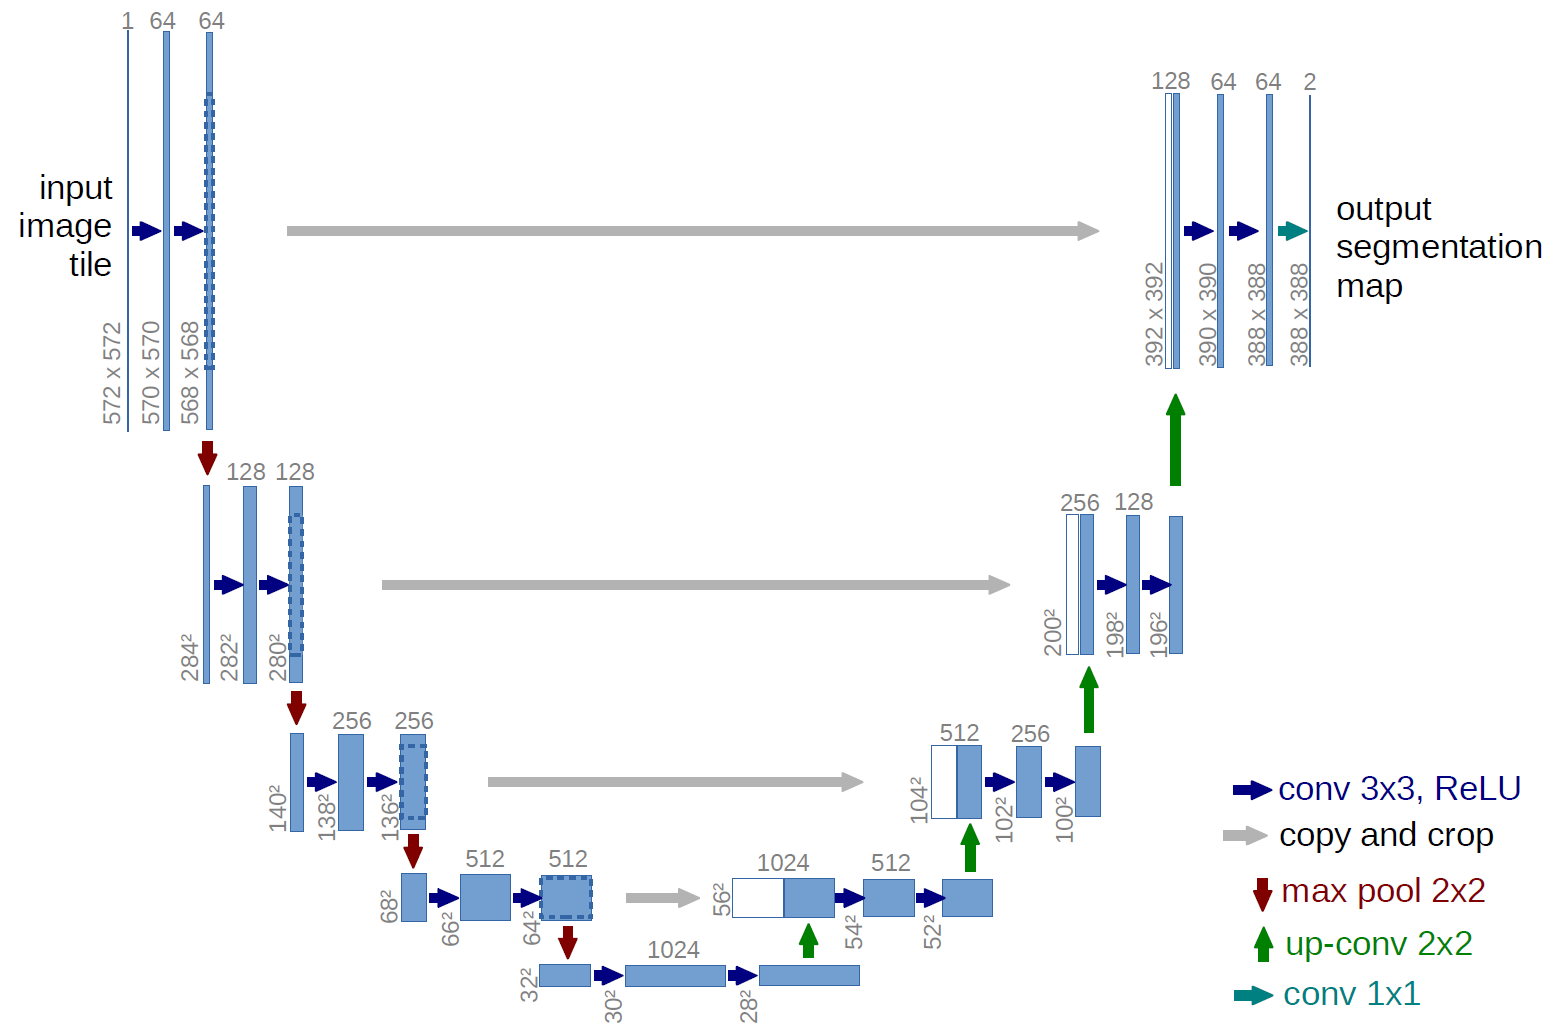
\includegraphics[scale=0.25]{images/u-net-architecture.png}
    \caption{U-net architecture (example for 32x32 pixels in the lowest resolution). Each blue box corresponds to a multi-channel feature map. The number of channels is denoted on top of the box. The x-y-size is provided at the lower left edge of the box. White boxes represent copied feature maps. The arrows denote the different operations.}
    \label{fig:u-net-architecture}
\end{figure}

The first part of the architecture - the \textbf{contractive path} - captures the global context of the image and reduces the sizes, identifying the relevant features in the input image. It consists of the repeated application of convolutions 3x3, each followed by a max 2x2 pooling operation for downsampling.\\

The second part of the architecture - the \textbf{expansive path} - creates a high-resolution segmentation map of the original image and enables precise localization (combining high-resolution features from the contracting path and the upsampled output of this phase). Each step consists of an upsampling of the feature map followed by a 2x2 convolution ("up-convolution", a concatenation with the corresponding cropped feature map from the contracting path, and two 3x3 convolutions, to increase the resolution. The upsampling part has a large number of feature channels, allowing the network to propagate context information to higher-resolution layers. The skip connections help to recover the spatial information lost in the contracting path, helping to locate the features more accurately.\\

At the final layer, a 1x1 convolution is used to map each 64-component feature vector to the desired number of classes. So, each pixel in the output image represents a label that corresponds to a particular object or class in the input image. In this case, the output map is a binary segmentation map where each pixel represents a foreground or background region.\\

This architecture is particularly suitable for semantic segmentation in the medical field because it is effective even with a limited dataset and a higher accuracy.

%%%%%%%%%%%%%%%%%%%%%
\subsection{UNETR}

UNETR\cite{hatamizadeh2022unetr}, or UNEt TRansformer, is a transformer-based architecture for medical image segmentation. This architecture utilizes a pure vision transformer as the encoder to capture the global contextual representations using the U-shape of the UNet architecture \cite{ronneberger2015u} but without relying on CNNs for feature extraction. The CNN-based decoder, connected with the encoder via skip connections, combines the extracted representations at different resolutions and predicts the segmentation output.\\

It was introduced to overcome the problem in FCNN-based approaches, in which the localized receptive fields limit the learning capabilities to relatively small regions without learning long-range dependencies, resulting in sub-optimal segmentations.\\
Transformer models, created mainly for Natural Language Processing tasks, have been applied to various tasks. Compared to FCNN models, they can model and learn long-range information and capture the global context using a sequence of 1D patch embeddings (as the word sequences in NLP).

In this paper, they used a transformer for a 3D medical image segmentation task seeing it as a 1D sequence-to-sequence prediction, learning contextual information from the embedded input patches. Combining the transformer-based encoder and the CNN-based decoder, they can properly capture both global and localized information.

\begin{figure}[H]
    \centering
    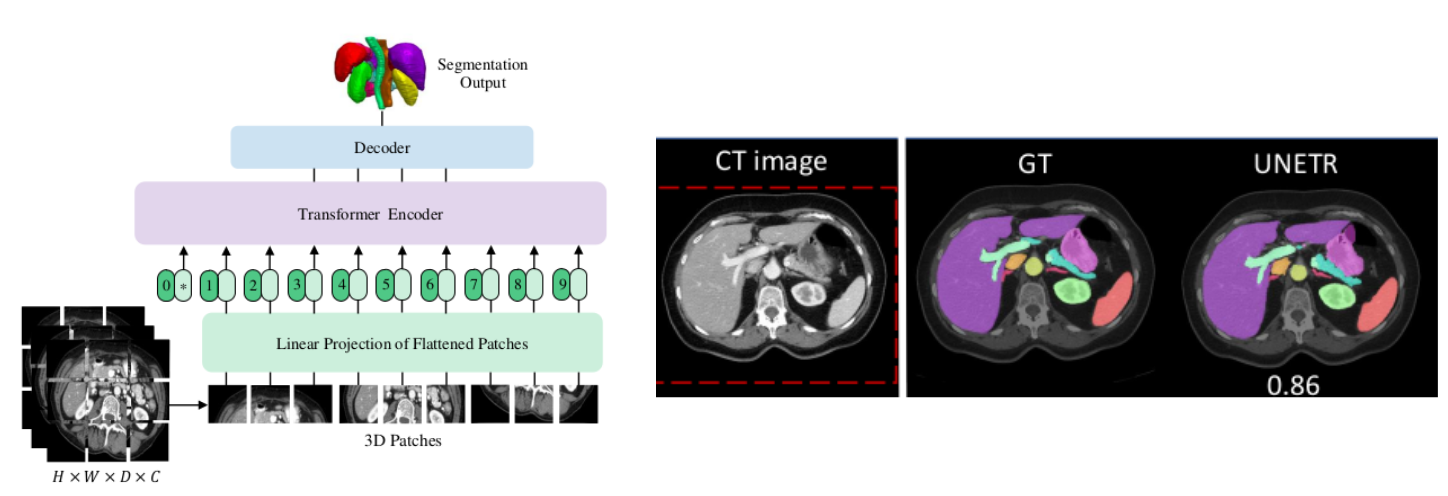
\includegraphics[scale=0.3]{images/unetr_1.png}
    \caption{General architecture of UNETR and an example of possible results from BTCV challenge dataset \cite{landman2015miccai}}
    \label{fig:unetr1-architecture}
\end{figure}

To pass the input to the encoder, the 3D input volume is partitioned into a series of consistent and non-overlapping patches. These patches are then projected into an embedding space through the application of a linear layer. Following this, the sequence is augmented with a positional embedding and serves as the input for the transformer encoder.
The transformer model encodes representations across various layers, and these encoded representations are subsequently extracted and combined with a decoder through skip connections to maintain at the end the same size as the input. This process is essential for predicting the output segmentation.

\begin{figure}[H]
     \centering
     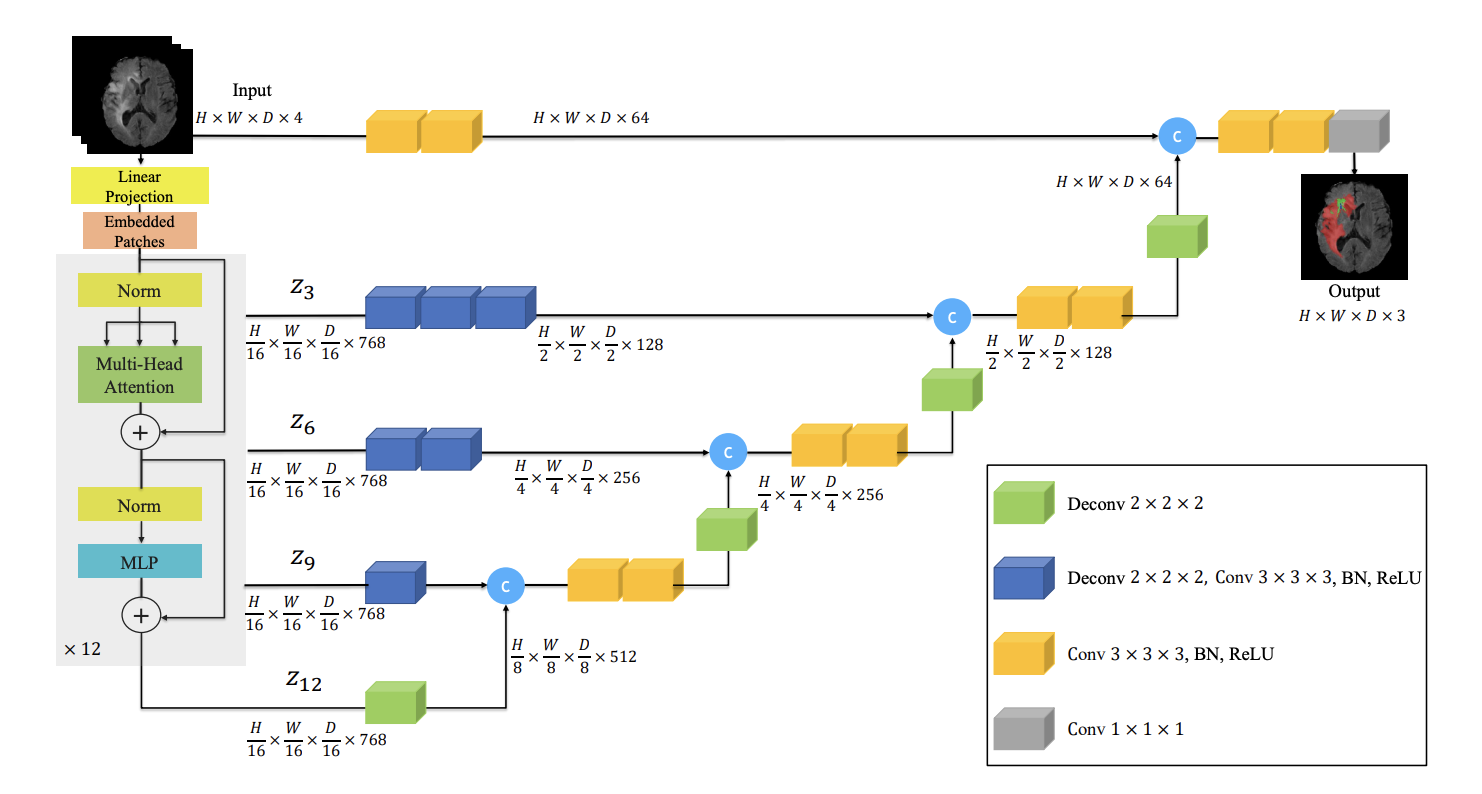
\includegraphics[scale=0.6]{images/unetr2.png}
     \caption{UNETR architecture details}
     \label{fig:unetr2-architecture}
\end{figure}


%%%%%%%%%%%%%%%%%%%%%
\subsection{Masked Autoencoders}

Masked Autoencoders (MAE) \cite{he2022masked}  are a type of autoencoder neural network architecture designed for self-supervised learning and feature representation. Autoencoders, in general, aim to learn meaningful compressed representations of input data. The core idea behind MAEs is the introduction of a masking mechanism to the traditional autoencoder structure to learn more meaningful and lower-dimensional representations and use them to reconstruct missing or masked portions of input images.

\begin{figure}[H]
    \centering
    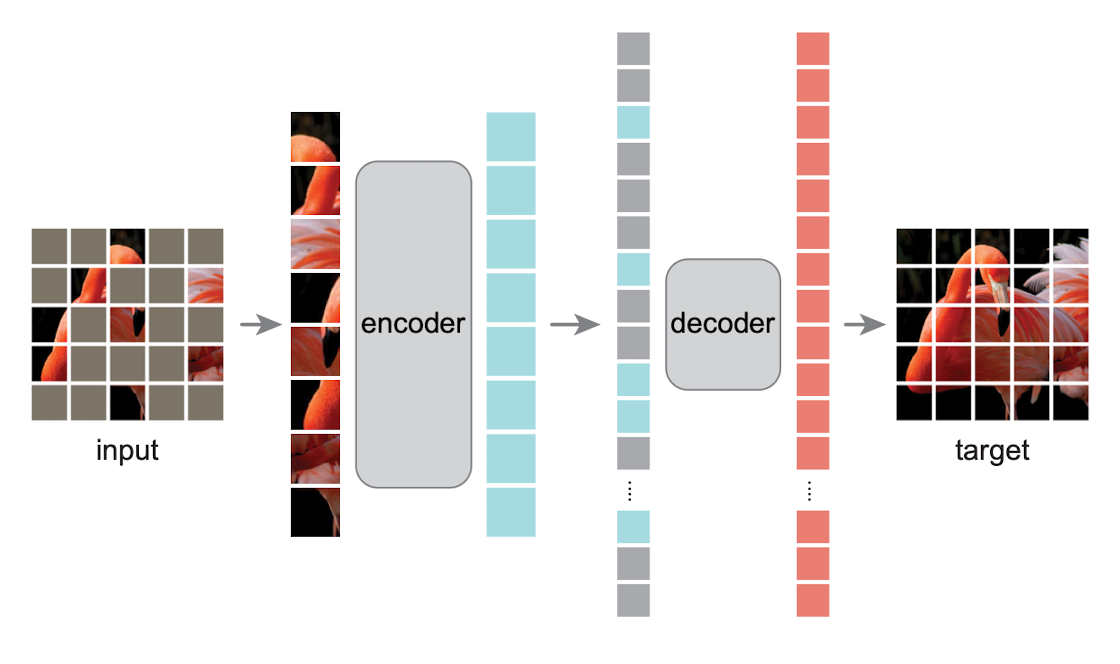
\includegraphics[scale=0.25]{images/mae1.png}
    \caption{MAE Architecture}
    \label{fig:mae1-architecture}
\end{figure}

The architecture consists of an asymmetric encoder-decoder setup. The ViT encoder takes the input data and applies to them a masking mechanism, which selectively ignores or sets certain elements to zero masking portions of the input images.
The encoder processes only the visible subset of patches (without mask tokens), mapping it to a lower-dimensional representation.
The decoder reconstructs the entire image from the latent representations and mask tokens (adding positional embeddings to have location information). The masking information is propagated through the decoding process to ensure that only the relevant information is used in the reconstruction.\\

Training involves minimizing the reconstruction loss, which encourages the encoder to learn useful features, strengthened by the masking mechanism. Regularization terms can be added to encourage sparsity in the latent space, promoting a more compact and meaningful representation.\\
The authors found that masking a high proportion of the input image, e.g., 75\%, yields a nontrivial and meaningful self-supervisory task, allowing also the model to generalize very well training with only a fraction of compute and memory.\\

Moreover, this network exhibits remarkable adaptability to diverse tasks. The MAE decoder is only used during pre-training to perform the image reconstruction task. Then a big advantage in this architecture lies in the flexibility of the decoder architecture, as it can be effortlessly modified independently of the encoder design.

%%%%%%%%%%%%%%%%%%%%%%%%%%%%%%%%%%%%%%%%%%%
\subsection{MAE+UNetr}
Our approach begins with an MAE encoder, which maps the input image into a latent space, capturing intermediary representations along the way. This latent space serves as input to the MAE decoder, which reconstructs the original image. Subsequently, we utilize the original image, the latent space, the intermediary representations, and the reconstructed images as input to a U-NetR decoder. The U-NetR decoder generates a segmentation mask, allowing us to extract meaningful features and enhance the segmentation performance.

\begin{figure}[H]
    \centering
    \includesvg[scale=0.7]{images/arch.svg}
    \caption{MAE+UNETR architecture}
    \label{fig:complete-arch}
\end{figure}

% \begin{figure}[H]
%     \centering
%     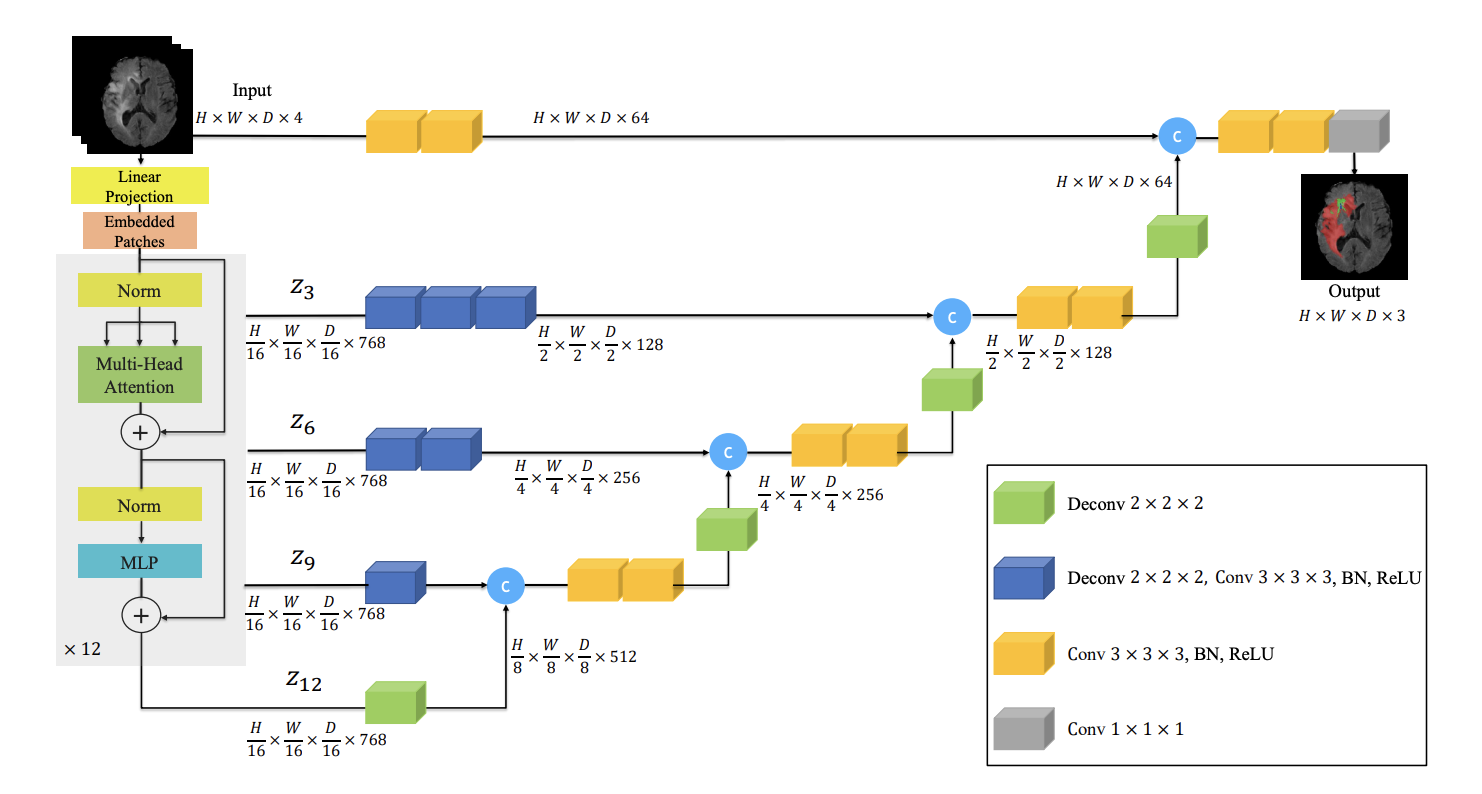
\includegraphics[scale=0.5]{images/unetr2.png}
%     \caption{UNETR architecture - 2}
%     \label{fig:unetr2-architecture}
% \end{figure}